%!TeX program=pdflatex
%!TeX encoding=utf8
%!TeX spellcheck = en_US
%!TeX root = ../../messageVortex.tex

\partepigraph{It was the anonymity. He wanted to be unknown, unpossessed by others' knowledge of him. That was freedom.}{Ling Ma, Severance}
\part{Anonymous Communication Systems\label{sec:systems}}
\chapter{Well Known Standard Protocols}
\section*{SMTP and Related Post Office Protocols (1982)}
Today's mail transport is mostly done via \defref{SMTP}\index{SMTP} protocol, as specified in \cite{RFC5321}. This protocol has proven to be stable and reliable. Most of the messages are passed from an MUA to an SMTP relay of a provider. From there, the message is directly sent to the SMTP server of the recipient and subsequently to the server-based storage of the recipient. The recipient may, at any time, connect to his server-based storage and may optionally relocate the message to a client-based (local) storage. The delivery from the server storage to the MUA of the recipient may happen by message polling or by message push (whereas the latter is usually implemented by a push-pull mechanism).

To understand the routing of a mail, it is essential to understand the whole chain starting from a user(-agent) until arriving at the target user (and being read!). To simplify this, we used a consistent model that includes all components (server and clients). The figure \ref{fig:MailAgents} shows all involved parties of a typical mail routing. It is essential to understand that mail routing remains the same regardless of the client. However, the availability of a mail at its destination changes drastically depending on the type of client used. Furthermore, control of the mail flow and control is different depending on the client.

The model has three main players storage (\defref{Storage}), agent (\defref{Agent}) and service (\defref{Service}). Storages are endpoint facilities storing emails received. Not explicitly shown are temporary storages such as spooler queues or state storages. Agents are simple programs taking care of a specific job. Agents may be exchangeable by other similar agents. A service is a bundle of agents that is responsible for a specific task or task sets.

\begin{figure}[ht!]
	\centering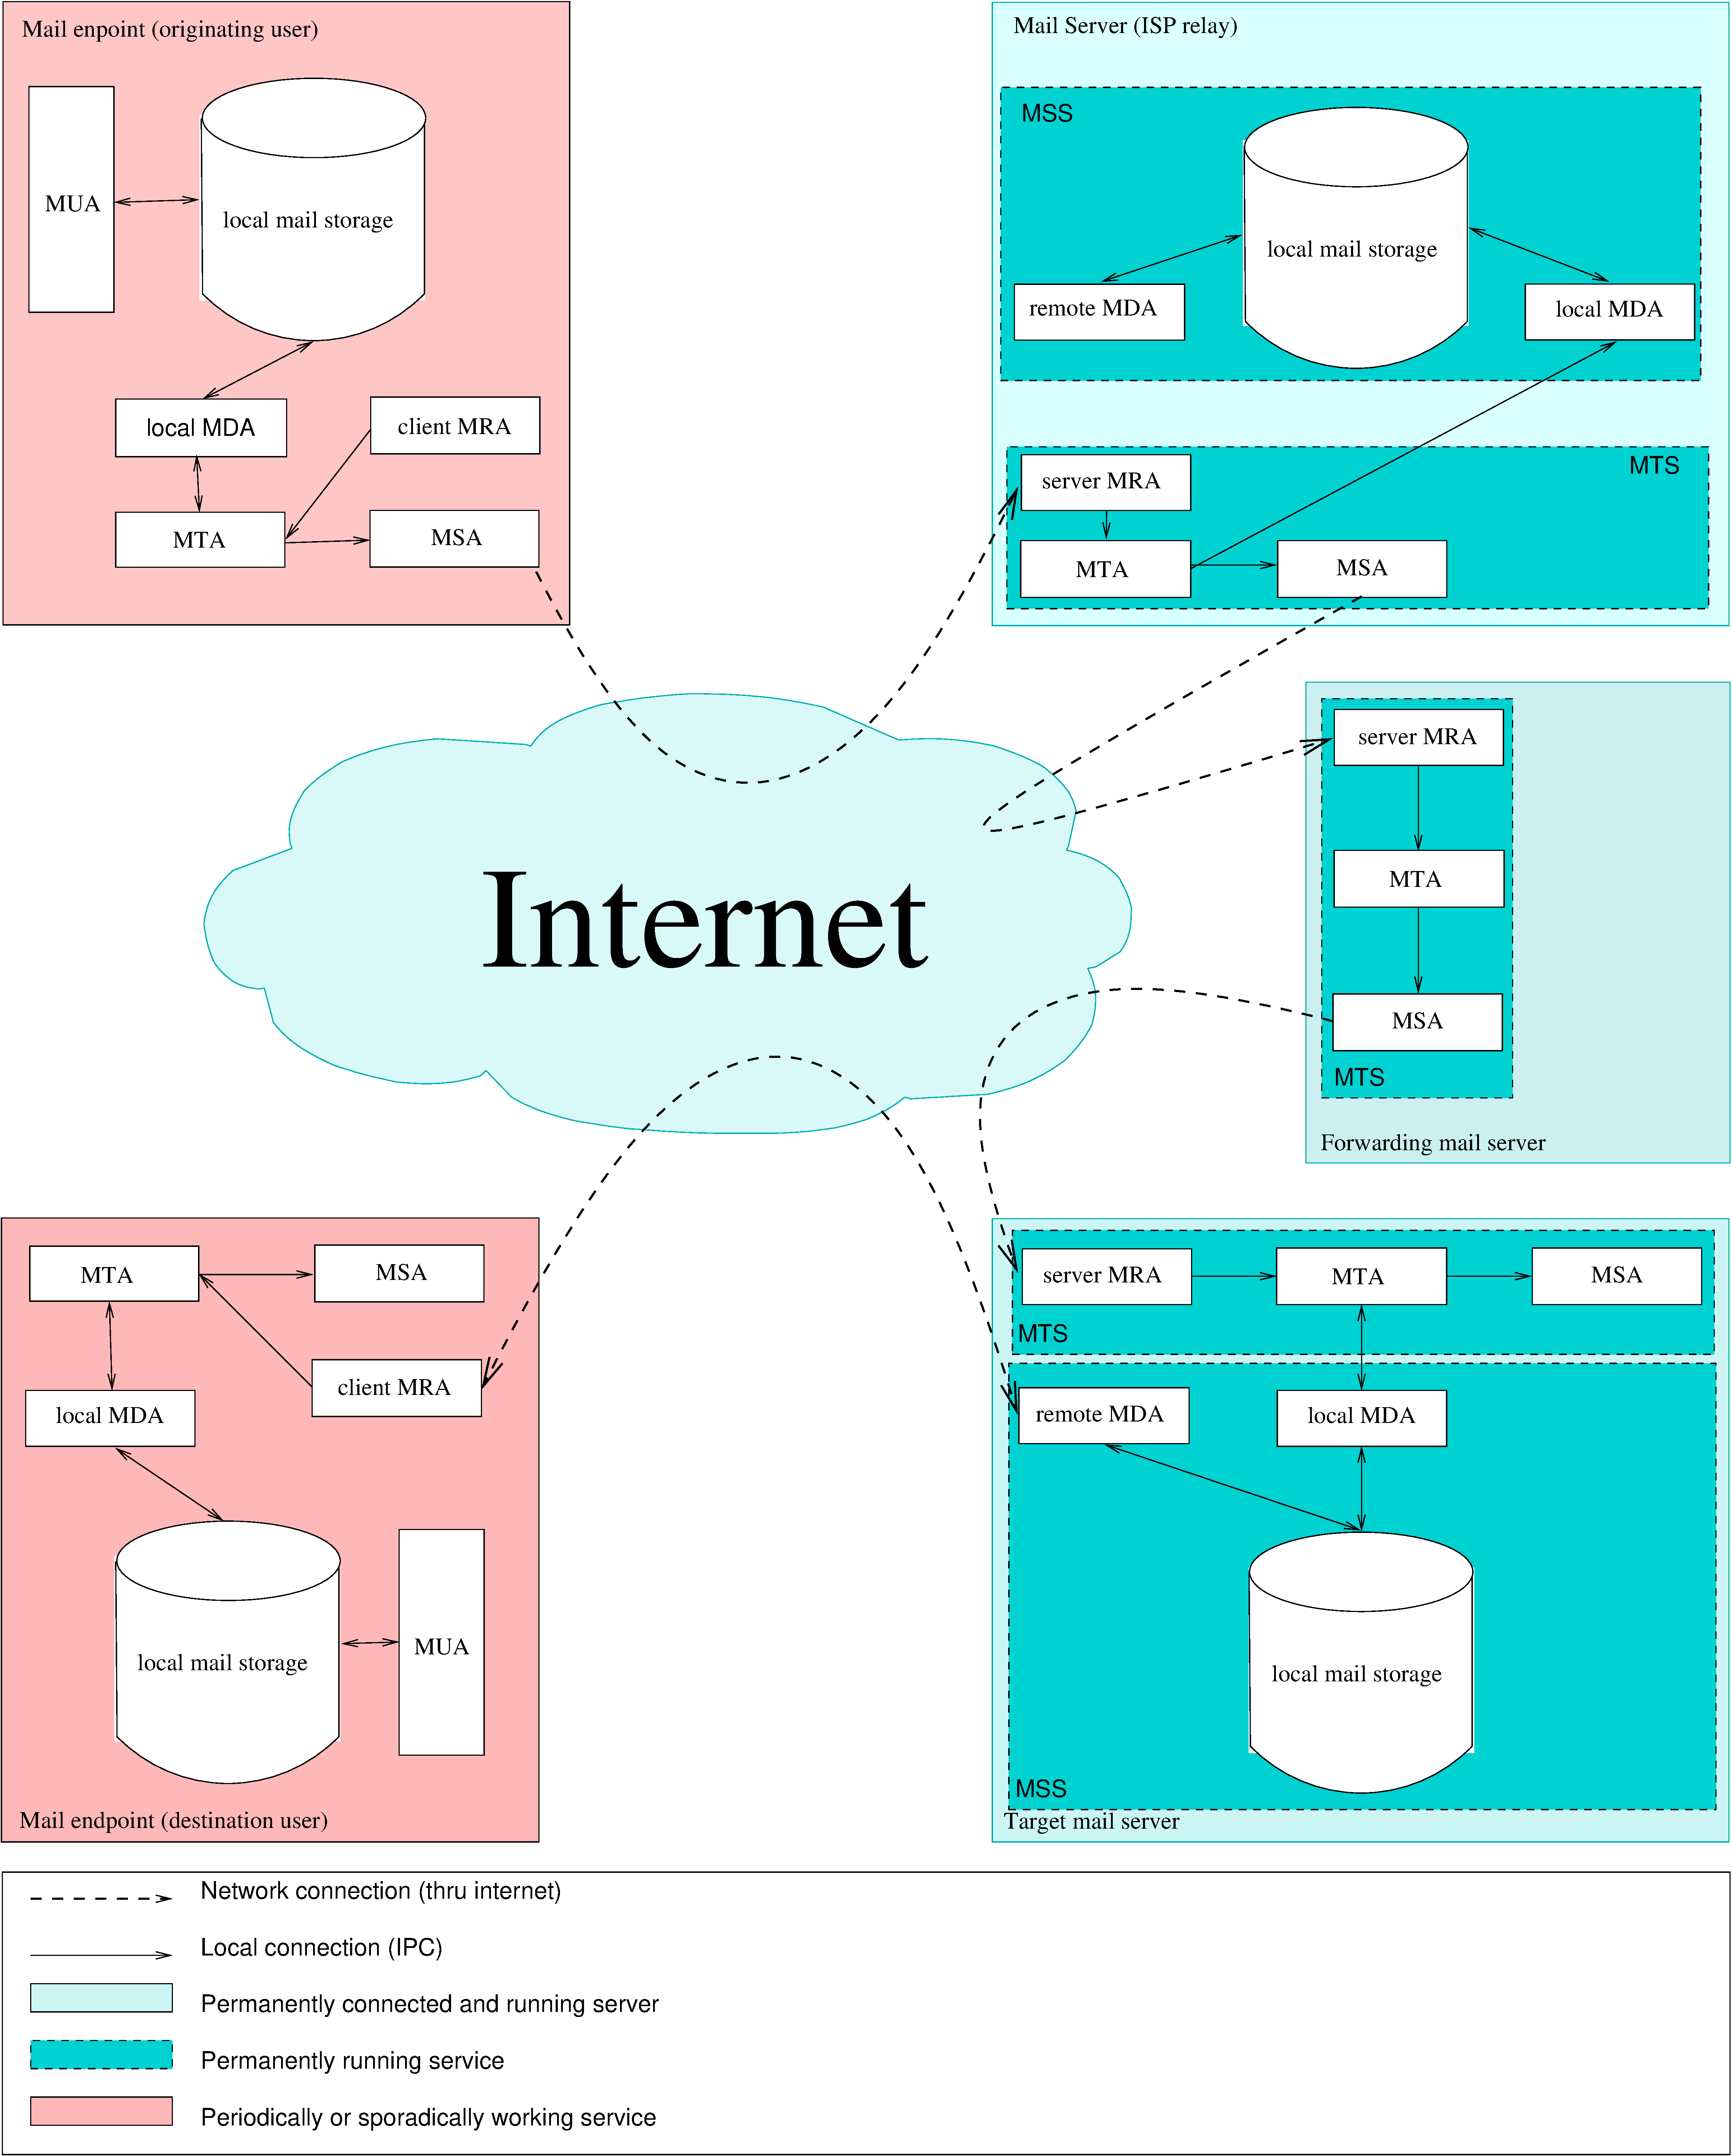
\includegraphics[width=\columnwidth]{inc/MailAgents1.pdf}
	\caption{Mail Agents}\label{fig:MailAgents}
\end{figure}

In the following paragraphs (for definitions), the term ``email'' is used synonymously to the term ``Message''.  ``Email'' has been chosen over ``messages'' because of its frequent use in standard documents.

Emails are typically initiated by a Mail User Agent (\defref{MUA}). An MUA accesses local email storage, which may be the server storage or a local copy. The local copy may be a cache only copy, the only existing storage (when emails are fetched and deleted from the server after retrieval), or a collected representation of multiple server storages (cache or authoritative).

Besides the MUA, the only other component accessing local email storage is the Mail Delivery Agent (\defref{MDA}). An MDA is responsible for storing and fetching emails from the local mail storage. Emails destined for other accounts than the current one are forwarded to the MTA. Emails destined to a User are persistently stored in the local email storage. It is essential to understand that email storage does not necessarily reflect a single mailbox. It may as well represent multiple mailboxes (e.g., a rich client-serving multiple IMAP accounts) or a combined view of multiple accounts (e.g., a rich client collecting mail from multiple \defref{POP} accounts). In the case of a rich client, the local MDA is part of the software provided by the user agent. In the case of an email server, the local MDA is part of the local email store (not necessarily of the mail transport service).

On the server-side, there are usually two components (services) at work. A ``Mail Transport Service'' (\defref{MTS}) responsible for mail transfers and a ``Mail Storage System'' which offers the possibility to store received Mails in a local, persistent store.\par

An MTS generally consists out of three parts. For incoming connects, there is a daemon called Mail Receiving Agent (\defref{Server MRA}) is typically a \defref{SMTP} listening daemon. A Mail Transfer Agent (\defref{MTA}) which is responsible for routing, forwarding, and rewriting emails. Moreover, a Mail Sending Agent (\defref{MSA}) which is responsible for transmitting emails reliably to another Server MRA (usually sent via \defref{SMTP}).\par

An MSS consists of local storage and delivery agents which do offer uniform interfaces to access the local store. They do also deal with replication issues, and grant should take care of the atomicity of transactions committed to the storage. Typically there are two different kinds of \defref{MDA}s. \defref{Local MDA}s offer possibilities to access the store via efficient (non-network based) mechanisms (e.g., IPC or named sockets). This is usually done with a stripped-down protocol (e.g., \defref{LMTP}). For remote agents there a publicly -- network-based -- agent available. Common Protocols for this \defref{Remote MDA}\ include \defref{POP}, \defref{IMAP}, or \defref{MS-OXCMAPIHTTP}.\par

Mail endpoints consist typically of the following components:
\begin{itemize}
	\item A Mail User agent (\defref{MUA})
	\item A Local Mail storage (\defref{MUA})
	\item A Local Mail Delivery Agent (\defref{Local MDA})
	\item A Mail Transfer Agent (\defref{MTA})
	\item A Mail Sending Agent (\defref{MSA})
	\item A Mail Receiving Agent (\defref{MRA})
\end{itemize}

Only two of these components do have external interfaces. These are \defref{MSA} and \defref{MRA}. \defref{MSA} usually uses \defref{SMTP} as transport protocol. When doing so, there are a couple of specialties. 
\begin{itemize}
	\item Port number is 587 (specified in \cite{RFC4409}).\\
	Although port numbers 25 and 465 are valid and do usually have the same capabilities, they are for mail routing between servers only. Mail endpoints should no longer use them.
	\item Connections are authenticated.\\
	Unlike a normal server-to-server (relay or final delivery) SMTP connections on port 25, clients should always be authenticated of some sort. This may be based on data provided by the user (e.g., username/password or certificate) or data identifying the sending system (e.g., IP address)\cite{RFC4409}. Failure in doing authentication may result in this port being misused as a sender for \defref{UBM}.
\end{itemize}

Mail User Agents (MUA) are the terminal endpoint of email delivery. Mail user agents may be implemented as fat clients on a desktop or mobile system or as an interface over a different generic protocol such as HTTP (Web Clients). 

Server located clients are a special breed of fat clients. These clients share the properties of fat clients except for the fact that they do not connect to the server. The client application itself has to be run on the server where the mail storage persists. This makes delivery and communication with the server different. Instead of interfacing with an MSA and a client MDA, they may directly access the local mail storage on the server. On these systems, the local mail storage may be implemented as a database in a user-specific directory structure.

\subsubsection*{Fat clients}
The majority of mail clients are fat clients. These clients score over the more centralistic organized web clients in the way that they may offer mail availability even if an Internet connection is not available (through client-specific local mail storage). They furthermore provide the possibility to collect emails from multiple sources and store them in the local storage. Unlike Mail servers, clients are assumed to be not always online. They may be offline most of the time. To guarantee the availability of a particular email address, a responsible mail server for a specific address collects all emails (the \defref{MSS} does this) and provides a consolidated view onto the database when a client connects through a local or remote MDA.

As these clients vary heavily, it is mandatory for the MDA that they are well specified. Lack of doing so would result in massive interoperability problems. Most commonly the Protocols \defref{IMAP}, \defref{POP} and \defref{EWS} are being used these days. For email delivery, the SMTP protocol is used. 

Fat clients are commonly used on mobile devices. According to  \cite{clientDistribution} in Aug 2012 the most typical fat email client was Apple Mail client on iOS devices ($35.6\%$), followed by Outlook ($20.14\%$), and Apple Mail ($11\%$). \citetitle{clientDistribution2}\cite{clientDistribution2} as a more recent source lists in February 2014 iOS devices with $37\%$, followed by Outlook ($13\%$), and  Google Android ($9\%$).

\subsubsection*{Server located clients}
Server located clients build an absolute minority. This kind of clients was common in the days of centralized hosts. An example for a Server Located Client is the Unix command ``mail''. This client reads email storage from a file in the users home directory.

\subsubsection*{Web clients}
Web clients are these days a common alternative to fat clients. Most big provider companies use their proprietary web client. According to \cite{clientDistribution2} the most common web clients are "`Gmail"', "`Outlook.com"', and "`Yahoo! Mail"'. All these Interfaces do not offer a kind of public plug-in interface. However,  they do offer IMAP-interfaces. This important for a future generalistic approach to the problem.

\section*{S/MIME (1996)}
S/MIME is an extension to the MIME standard. The MIME standard allows in simple text-oriented mails an alternate representation of the same content (e.g., as text and as HTML), or it allows to split a message into multiple parts that may be encoded. It is important to note that MIME encoding is only effective in the body part of a mail.

S/MIME, as described in \cite{RFC3851}, extends this standard with the possibility to encrypt mail content or to sign it. Practically this is achieved by either putting the encrypted part or the signature into an attachment. It is essential to know that this method leaks significant pieces of the data.

As the mail travels directly from sender to recipient, both involved parties are revealed. Neither message subject nor message size or frequency is hidden. This method does offer limited protection when assuming an adversary with interest in the message content only. It does not protect from the kind of adversary in our case. 

The trust model is based on a centralistic approach involving generally trusted root certification authorities.

\section*{Pretty Good Privacy (1996)}
Exactly as S/MIME, PGP\cite{rfc4880} builds upon the base of MIME. Although the trust model in PGP is peer-based. The encryption technology does not significantly differ (as seen from the security model).

Like S/MIME, PGP does not offer anonymity. Sender and endpoints are known to all routing nodes. Depending on the version of PGP, some meta-information or parts of the message content such as subject line, the real name of the sender and receiver, message size is leaked.

A good thing to learn from PGP is that peer-based approaches are offering limited possibilities for trust. The trust in PGP is based on the peer review of users. This peer review may give an idea of how well verified the key of a user is.


\chapter{Information Routing and Distribution for Anonymizing Protocols}
Information routing and distribution is not a novelty in privacy research. Researchers arround the globe have searched for means of privacy.  One good example was the patent in the intro of Almon B. Strowger\cite{pulseDialingPatent}. More recent activities are the  infamous "How to share a secret"\cite{shamir1979share}, which used Lagrange polynomials to distribute shares of information accross multiple hosts for privacy. A single polynomial would be attackable. Therefore Shamir applied a $\mod p$ operation to hide characteristics of a curve (as long as $p$ is large and prime). The system had many problems which were addressed by subsequent work such as \cite{tompa1989share}.

Lagrange polynomes form an important part when it comes to networking and privacy. They are commonly used in the form of Reed-Solomon codes for securing unreliable connections (e.g., \cite{aiache2008reed}), distributing data \cite{shamir1979share}.

Our approach will be to use Lagrange not primarily for distributing data but to generate unidentifiable decoy traffic. When applying a Lagrange polynomial to a message all factors contain parts of the original message. Given enough factors of the polynomial, anyone may reconstruct the original message. As a result an adversary is not able which parts of the traffic is decoy and which part is message as all parts have the potential to recover the original message.

\section{Mixing\label{sec:mixNets}}
Mixes have been first introduced by \citetitle{CHAUM1}\cite{CHAUM1} in \citeyear{CHAUM1}. The basic concept in a mix goes as follows. We do not send a message directly from the source to the target. Instead, we use a kind of proxy server or router in between which picks up the packet, anonymizes it, and forwards it either to the recipient or another mix. If we assume that we have at least three mixes cascaded, we then can conclude that:
\begin{itemize}
	\item Only the first mix knows the true sender
	\item All intermediate mixes know neither the true sender nor the true recipient (as the data comes from mixes and is forwarded to other mixes) 
	\item Only the last mix knows the final recipient.
\end{itemize}

This approach (in this simple form) has several downsides and weaknesses.

\begin{itemize}
	\item In a low latency network, the message may be traced by analyzing the timing of a message.
	\item We can emphasize a path by replaying the same message multiple times (assuming we control an evil node), thus discovering at least the final recipient.
	\item If we can ``tag'' a message (with content or attribute), we then may be able to follow the message.
\end{itemize}

In \citeyear{RP03-1} \citeauthor{RP03-1} analyzed the suitability for mixes as an anonymizing network for masses. They concluded that there are three possibilities to run mixes.
\begin{itemize}
	\item Commercial, static MixNetworks
	\item Static MixNetworks operated by volunteers
	\item Dynamic MixNetworks
\end{itemize}
They concluded that in an ideal implementation, a dynamic mix network where every user is operating a mix is the most promising solution as static mixes always might be hunted by an adversary.

\section{Anonymous Remailers\label{sec:remailers}}
Remailers have been in use for quite some time. There are several classes of remailers, and all of them are somehow related to Mixnets. There are ``types'' of remailers defined. Although these ``types'' offer some hierarchy, none of the more advanced ``types'' seem to have more than one implementation in the wild. 

Pseudonymous Remailers (also called Nym Servers) take a message and replace all information pointing to the original sender with a pseudonym. This pseudonym may be used as an answer address. The most well known pseudonymous remailer possibly was anon.penet.fi run by Johan Helsingius. This service has been forced several times to reveal a pseudonyms true identity before Johan Heösingius decided to shut it down. For a more in-depth discussion of Pseudonymous Remailers see \ref{sec:remPseudo}

Cypherpunk remailers forward messages like pseudonymous remailers. Unlike pseudonymous remailers, Cypherpunk remailers decrypt a received message, and its content is forwarded without adding a pseudonym. A reply to such a message is not possible. They may, therefore, be regarded as an ``decrypting reflector'' or a ``decrypting mix'' and may be used to build an onion routing network for messages. For a more in-depth discussion of type-1-remailers, see section  \ref{sec:remCypherpunk}.

Mixmaster remailers are very similar to Cypherpunk remailers. Unlike them, Mixmaster remailers hide the messages, not in an own protocol, but use \defref{SMTP} instead. While using \defref{SMTP} as a transport layer, Cypherpunk remailers are custom (non-traditional mail) servers listening on port 25. For a more in-depth discussion of type-2-remailers, see section \ref{sec:remMixmaster}.

Mixminion remailers extend the model of Mixmaster remailers. They still use \defref{SMTP} but introduce new concepts. New concepts in Mixminion remailers are:
\begin{itemize}
	\item Single Use Reply Blocks (SURBs)
	\item Replay prevention
	\item Key rotation
	\item Exit poicies
	\item Dummy traffic
\end{itemize}
For a more in depth discussion of Mixminion remailers see section \ref{sec:remMixminion}.


\section{Onion Routing}
Onion routing is a further development of the concept of mixes. In onion routers, every mix gets a message which is asymmetrically encrypted. By decrypting the message, he gets the name of the next-hop and the content which he has to forward. The main difference in this approach is that in traditional mix cascades, the mix decides about the next hop. In an onionised routing system, the message decides about the route it is taking. 

Onionized messages typically have the problem of a constant size loss throughout the system. Some systems counter this effect, y separating the routing setup from the message path.

While tagging attacks are far harder (if we exclude side-channel attacks to break sender anonymity), the traditional attacks on mixes are still possible. So when an adversary is operating entry and exit nodes, it is straightforward for them to match the respective traffic.

One very well known onion routing network is Tor (\href{https://www.torproject.org}{https://www.torproject.org}). For more information about Tor see section \ref{sec:tor}.

\section{Garlic Routing}
Grarlic routing is an improved form of onion routing. To stop onionized messages to continuosly loose contents through their way, a garlic router collects multiple, independent messages into one message before routing. This compensates for the ``size loss effect'' of onionized systems.

\section{Crowds}
Crowds is a network that offers anonymity within a local group. It works as follows:

\begin{itemize}
	\item All users add themselves to a group by registering on a so-called ``blender''.
	\item All users start a service (called JonDo).
	\item Every JonDo takes any received message (might be from him as well) and sends it with a 50\% chance either to the correct recipient or to a randomly chosen destination
\end{itemize}

While crowds as specified in \cite{crowds:tissec} does anonymize the sender from the recipient rather well, the system offers no protection from someone capable of monitoring crowds traffic. The system may, however, be easily attacked from within by introducing collaborating johndos. It has been further developed to D-Crowds \cite{crowdsAttack}, ADU/RADU \cite{Munoz-Gea2008}, Freenet\cite{freenet} and others. 

Furthermore, the blender is aware of all JonDos and thus of particular interest for any observing or censoring adversary. Control of the blender enables an adversary to split the network into controllable parts, adding a high likelihood of discovering an original sender.

\section{Mimic Routes}
Mimics are a set of statical mixes which maintain a constant message flow between the static routes. If legitimate traffic arrives, the pseudo traffic is replaced by legitimate traffic. An outstanding observer is thus incapable of telling the difference between real traffic and dummy traffic.

If centralized mixes are used, the system lacks the same vulnerabilities of sizing and observing the exit nodes as all previously mentioned systems. If we assume that the sender and receiver operate a mixer by themselves, the system would no longer be susceptible to timing or sizing analyses. The mimic routes put a constant load onto the network. This bandwidth is lost and may not be reclaimed. It does not scale well as every new participant increases the need for mimic routes and creates (in the case of user mixes) a new mimic load. Furthermore, the mixes are easily identifiable as their characteristic data stream contrasts compared to other network service streams.

\section{Distributed Hash Tables}
\fxwarning{complete section}

\section{Dining Cryptographer Networks}
DC networks are based on the work \citetitle{chaum-dc} by \citeauthor{chaum-dc}\cite{chaum-dc}. In this work, \citeauthor{chaum-dc} describes a system allowing a one-bit transfer (The specific paper talks about the payment of a meal). Although all participants of the DC net are known, the system makes it unable to determine who has been sending a message. The message in a DC-Net is readable for anyone. This network has the downside that a cheating player may disrupt communication without being traceable.

Several attempts have been made to strengthen the proposal of Chaum\cite{golle:eurocrypt2004,disco,herbivore:tr,Corrigan-Gibbs:2010:DAA:1866307.1866346}. However, no one succeeded without introducing significant downsides on the privacy side.

\chapter{Proposed Academic Protocols and System Implementations\label{sec:implSystems}}
\fxwarning{complete section}
\section{Characteristics of Known Anonymity Implementations}
Table \ref{tab:anonClass} shows the previously analyzed protocols.

\DeclareFixedFootnote{\takenFrom}{Definition taken from \ref{Shirazi2018}}
\begin{table*}[ht]\centering\tiny

	\label{tab:anonClass}
	\setlength{\aboverulesep}{0pt}
	\setlength{\belowrulesep}{0pt}
	\newcolumntype{x}[1]{!{\centering\arraybackslash\vrule width #1}}
	\gdef\mybull{\medbullet}
	\gdef\mycirc{\medcirc}
	\gdef\mytick{\faCheck}
	\gdef\mycross{\faTimes}
	% network
	%\usepackage{ amssymb }
	\newcommand\networkFully{$\boxtimes$}
	\newcommand\networkMostly{$\square$}
	\newcommand\networkPartly{$\sqsubset$}
	%direction
	\newcommand\directionBidi{$\longleftrightarrow$}
	\newcommand\directionUnidi{$\longrightarrow$}
	% synchronization
	\newcommand\syncAsync{$\neq$}
	\newcommand\syncSynchronous{$\cong$}
	% symmetry
	\newcommand\rolePtp{\scalebox{0.4}{$\mybull\cdot\cdot\mybull\cdot\cdot\mybull$}}
	\newcommand\roleCs{\scalebox{0.4}{$\mybull\cdot\cdot\mybull$}}
	\newcommand\roleHybrid{\scalebox{0.4}{$\mybull\cdot\cdot\mycirc\cdot\cdot\mybull$}}
	% Hierarchy
	\newcommand\hierarchyFlat{$\cdots$}
	\newcommand\hierarchyHierarchical{\ding{68}}
	% centralization
	\newcommand\decentralizationPart{\astrosun}
	\newcommand\decentralizationDecentr{$\bigcirc$}
 	\newcommand\decentralizationNo{\mycross}
	% Network view
	\newcommand\netviewFully{$\CIRCLE$}
	\newcommand\netviewPartly{$\LEFTcircle$}
	% NW updating
	\newcommand\updatingTimed{\clock}
	\newcommand\updatingEvent{\lightning}
	\newcommand\updatingNoupd{\mycross}
	% Routing
	\newcommand\routingRoutesrc{\scalebox{0.4}{$\mybull\cdots$}}
	\newcommand\routingRoutehop{\scalebox{0.4}{$\cdots\mybull\cdots$}}
	\newcommand\routingRoutebc{\faBullhorn}
	% Sheduling
	\newcommand\shedfair{$\equiv$}
	\newcommand\shedprio{$\Diamonddot$}
	%determinism
	\newcommand\nsdetdet{\mytick}
	\newcommand\nsdetprob{\mycross}
	%selection set
	\newcommand\nsnodesall{\CircledA}
	\newcommand\nsnodessec{\Stopsign}
	\newcommand\nsnodesnet{\Mundus}
	\newcommand\nsnodesusr{\smiley}
	% probability
	\newcommand\nsprobuni{$\circledast$}
	\newcommand\nsprobstat{$\circledcirc$}
	\newcommand\nsprobdyn{$\ast$}
	% latency
	\newcommand\perflatl{L}
	\newcommand\perflath{H}
	\newcommand\perflatm{M}
	% mode 
	\newcommand\perfmodecon{$\multimapdotboth$}
	\newcommand\perfmodemsg{\Letter}
	% implementation
	\newcommand\nsimplyes{\mytick}
	\newcommand\nsimplno{\mycross}
	% code available
	\newcommand\nscodeyes{\mytick}
	\newcommand\nscodeno{\mycross}
	% context
	\newcommand\nscontmsg{\faEnvelope}
	\newcommand\nscontmail{@}
	\newcommand\nscontbulletin{\faUsers}
	\newcommand\nscontphone{\Telefon}
	\newcommand\nscontwww{\faInternetExplorer}
	\newcommand\nscontmicroblog\faPencil
	\newcommand\nscontfiles\faStickyNote
	\newcommand\nscontwifi\faWifi
	\newcommand\nscontBC{\faBullhorn}
	\gdef\cwidth{0.36cm}
	\rowcolors{8}{black!30}{black!10}
	\begin{tabular}{x{2pt}lx{2pt}*{5}{p{\cwidth}|}p{\cwidth}x{2pt}p{\cwidth}|p{\cwidth}x{2pt}*{4}{p{\cwidth}|}p{\cwidth}x{2pt}*{4}{p{\cwidth}|}p{\cwidth}x{2pt}}
		\toprule
		
		& \multicolumn{6}{cx{2pt}}{Network Structure} & \multicolumn{2}{p{1.2cm}x{2pt}}{\centering Routing Information} & \multicolumn{5}{cx{2pt}}{Communication Model} & \multicolumn{5}{cx{2pt}}{Performance and Deployability}\\\cmidrule{2-19}
		
		& & \multicolumn{2}{c|}{Connection} & \multicolumn{3}{cx{2pt}}{Symmetry} & & & & & \multicolumn{3}{cx{2pt}}{Node Selection} & & & & & \\\cmidrule{3-4}\cmidrule{5-7}\cmidrule{12-14}
		
		& \rot{Topology} & \rot{Direction} & \rot{Synchronization} & \rot{Roles} & \rot{Hierarchy} & \rot{Decentralization} & \rot{Network view} & \rot{Updating} & \rot{Routing Type} & \rot{Scheduling} & \rot{Determinism} & \rot{Selection set} & \rot{selection probability} & \rot{Latency} & \rot{Communication mode} & \rot{Implementation} & \rot{Code availability} & \rot{Context/application} \\
		\midrule
		
		\MessageVortex & \networkFully & \directionBidi & \syncSynchronous & \rolePtp & \hierarchyFlat & \decentralizationDecentr & \netviewPartly &  \updatingEvent &  \routingRoutesrc & \shedfair & \nsdetprob & \nsnodesusr & \nsprobuni & \perflath & \perfmodemsg & \nsimplyes & \nscodeyes & \nscontmail \\
		
		Chaum Mixes\takenFrom & \networkFully & \directionUnidi & \syncAsync & \roleCs & \hierarchyFlat & \decentralizationNo & \netviewFully & \updatingNoupd & \routingRoutesrc & \shedfair & \nsdetdet &  \nsnodesall & \nsprobstat & \perflath & \perfmodemsg & \nsimplyes & \nscodeno & \nscontmail \\
		
		Babel\takenFrom & \networkFully & \directionUnidi & \syncAsync & \roleCs & \hierarchyFlat & \decentralizationPart & \netviewFully & \updatingNoupd & \begin{tabular}{@{}c@{}}\routingRoutesrc \\ \routingRoutehop\end{tabular} & \shedfair & \nsdetdet &  \nsnodesall & \nsprobuni & \perflath & \perfmodemsg & \nsimplno & \nscodeno & \nscontmail \\

		Mixmaster\takenFrom & \networkFully & \directionUnidi & \syncAsync & \roleCs & \hierarchyFlat & \decentralizationPart & \netviewPartly & \updatingNoupd & \routingRoutesrc & \shedfair & \nsdetprob &  \nsnodesall & \nsprobuni & \perflath & \perfmodemsg & \nsimplyes & \nscodeyes & \nscontmail \\

		Mixminion\takenFrom & \networkFully & \directionUnidi & \syncAsync & \roleCs & \hierarchyFlat & \decentralizationPart & \netviewFully & \updatingTimed & \routingRoutesrc & \shedfair & \nsdetprob &  \nsnodesall & \nsprobuni & \perflath & \perfmodemsg & \nsimplyes & \nscodeyes & \nscontmail \\

		Tor\takenFrom & \networkPartly & \directionBidi & \syncSynchronous & \roleHybrid & \hierarchyFlat & \decentralizationPart & \netviewFully & \updatingTimed & \routingRoutesrc & \shedfair & \nsdetprob &  \nsnodesnet \nsnodessec & \nsprobstat & \perflatl & \perfmodemsg & \nsimplyes & \nscodeyes & \nscontwww \\

		Crowds\takenFrom & \networkFully & \directionBidi & \syncAsync & \rolePtp & \hierarchyFlat & \decentralizationPart & \netviewFully & \updatingEvent & \routingRoutehop & \shedfair & \nsdetprob &  \nsnodesall & \nsprobuni & \perflatl & \perfmodemsg & \nsimplyes &\nscodeno & \nscontwww \\

		MorphMix\takenFrom & \networkPartly & \directionBidi & \syncAsync & \rolePtp & \hierarchyFlat & \decentralizationPart & \netviewPartly & \updatingEvent & \routingRoutehop & \shedfair & \nsdetprob &  \nsnodesnet & \nsprobdyn & \perflatl & \perfmodecon & \nsimplyes & \nscodeyes  & \nscontwww \\

		Tarzan\takenFrom & \networkMostly & \directionBidi & \syncAsync & \rolePtp & \hierarchyFlat & \decentralizationDecentr & \netviewFully & \updatingEvent & \routingRoutesrc & \shedfair & \nsdetprob &  \nsnodessec  & \nsprobuni & \perflatl & \perfmodecon & \nsimplyes & \nscodeyes  & \nscontwww \\

		Torsk\takenFrom & \networkPartly & \directionBidi & \syncAsync & \roleHybrid & \hierarchyFlat & \decentralizationPart & \netviewPartly & \updatingEvent & \routingRoutesrc & \shedfair & \nsdetprob &  \nsnodesnet  & \nsprobuni & \perflatl & \perfmodecon & \nsimplyes & \nscodeno  & \nscontwww \\

		AP3\takenFrom & \networkPartly & \directionBidi & \syncAsync & \rolePtp & \hierarchyFlat & \decentralizationDecentr & \netviewPartly & \updatingEvent & \routingRoutehop & \shedfair & \nsdetprob &  \nsnodesall  & \nsprobuni & \perflatl & \perfmodecon & \nsimplno & \nscodeno  & \begin{tabular}{@{}c@{}}\nscontwww\nscontmail \\ \nscontBC \end{tabular}\\

		Salsa\takenFrom & \networkPartly & \directionBidi & \syncAsync & \begin{tabular}{@{}c@{}}\rolePtp \\ \roleHybrid \end{tabular} & \hierarchyFlat & \decentralizationDecentr & \netviewPartly & \updatingEvent & \routingRoutehop & \shedfair & \nsdetprob &  \nsnodesall  & \nsprobuni & \perflatl & \perfmodecon & \nsimplyes & \nscodeno & \nscontwww \\
		
		Chaum\'{}s DCnet\takenFrom & \networkFully & \directionUnidi  & \syncAsync & \rolePtp & \hierarchyFlat & \decentralizationNo & \netviewFully & \updatingEvent & \routingRoutebc & \shedfair & \nsdetdet & \nsnodesall & \nsprobstat & \perflath & \perfmodemsg & \nsimplno & \nscodeno & \nscontmsg \\

		Herbivore\takenFrom & \networkPartly & \directionUnidi  & \syncAsync & \rolePtp & \hierarchyHierarchical & \decentralizationPart & \netviewPartly & \updatingEvent & \routingRoutebc & \shedfair & \nsdetdet & \nsnodesnet & \nsprobstat & \perflatm & \perfmodemsg & \nsimplyes & \nscodeno & \nscontmsg \\

		Dissent in numbers\takenFrom & \networkPartly & \directionUnidi  & \syncAsync & \roleCs & \hierarchyHierarchical & \decentralizationPart & \netviewPartly & \updatingEvent & \routingRoutebc & \shedfair & \nsdetdet & \nsnodesnet & \nsprobstat & \perflath & \perfmodemsg & \nsimplyes & \nscodeyes & \nscontmsg \\

		$I^2P$\takenFrom & \networkMostly & \directionUnidi  & \syncAsync & \rolePtp & \hierarchyFlat & \decentralizationDecentr & \netviewFully & \updatingTimed & \routingRoutesrc & \shedprio & \nsdetprob & \nsnodesnet \nsnodessec & \nsprobdyn & \perflatl & \perfmodecon & \nsimplyes & \nscodeyes & \begin{tabular}{@{}c@{}} \nscontwww \nscontmail \\ \nscontfiles\end{tabular} \\

		$\mathcal{P}^5$\takenFrom & \networkPartly & \directionUnidi  & \syncAsync & \rolePtp & \hierarchyHierarchical & \decentralizationPart & \netviewPartly & \updatingEvent & \routingRoutebc & \shedprio & \nsdetdet & \nsnodesusr & \nsprobstat & \perflath & \perfmodemsg & \nsimplyes & \nscodeno & \nscontmsg\\
		
		Riffle & & & & & & & & & & & & & & & & & & \\

		Atom & & & & & & & & & & & & & & & & & & \\
		Riposte & & & & & & & & & & & & & & & & & & \\
		Pung & & & & & & & & & & & & & & & & & & \\
		PIR & & & & & & & & & & & & & & & & & & \\
		Karaoke & & & & & & & & & & & & & & & & & & \\
		Loopix & & & & & & & & & & & & & & & & & & \\
		Stadium & & & & & & & & & & & & & & & & & & \\
		Vuvuzela & & & & & & & & & & & & & & & & & & \\
		\bottomrule
	\end{tabular}
	\caption{Classification table for anonymization protocols according to \cite{Shirazi2018}}
\end{table*}
\section{Resenders, Onion Routers, and MixNets\label{sec:remailersAndMixnets}}
\subsection{Pseudonymous Remailers (1981)\label{sec:remPseudo}}
A pseudonymous remailer allows to reach people via a pseudonymous email address. On the remailing server all traces of the original sender are removed and a pseudonymous email is inserted instead. The foundation of these reamilers can be found in an early article of David Chaum\cite{CHAUM1}.

One of the most famous remailers was the Penet remailer (anon.penet.fi). This remailer only lasted from 1993 to 1996 and was shut down after at least two compromises involving the Chruch of Scientology. Details of the closure can be found in \cite{penetClosure}.

\subsection{Cypherpunk Remailers (approx. 1993)\label{sec:remCypherpunk}}
With the failing of anon.penet.fi, it became clear that the weakest spot of a single server infrastructure the information stored on the server and the vulnerability of their owner. The new type-1-remailers score over the existing type-0-remailers by using encryption for the message. Most of the time PGP was used and custom programmed mail processors on systems to achieve the functionallity. It is unclear when first type-1-remailers were invented. Setting up a type-1-remailer was typically achieved by using procmail together with a small script calling PGP binaries and then sending the resulting message to the next recipient. By combining multiple type-1-remailers, an onion-like structure of the message was achievable. 

This approach was promising, but it was still observable. An observation was possible by correlating the message sizes (e.g., strictly decreasing) and timing information. Furthermore, remailers were however still known and authorities were able to ban infrastructure and capable of monitoring their routing activities. Additionally, those remailers allowed to prosecute administrators of such systems.

\subsection{Babel (1996)}
Babel was an academic system defined in a paper by \citeauthor{babel} in \citeyear{babel}\cite{babel}. It has been developed at IBM Zurich Research Laboratory. It was a mixing system using onionized addresses. The sender remains anonymous while he may provide a reply routing block called RPI. If both parties would like to remain anonymous, the RPI of the initiator is deployed in a forum thread. Anyone using this block adds an RPI for its address to the message.

This system has all the disadvantages of a system using MURBs. Traffic highlighting and similar attacks are possible.

\subsection{Mixmaster-Remailers (1996)\label{sec:remMixmaster}}
Like Cypherpunk remailers, the Mixmaster remailers were working with onion-like encrypted messages. The protocol was based on Mix-Nets described by Chaum in \cite{CHAUM1} and further developed by L. Cotrell in 1996. 

In contrast to type-1-remailers, the use of cascading systems to remail became systematic. The enduser used specialized software to build and send Mixmaster messages.

Mixmaster messages were still traceable by message size. Reply blocks were not supported by the system. A user had to know all Mixmaster nodes in order to use the system. The last node was typically an exit node sending the message in clear to the final recipient. This behavior still allowed the use of Usenet.

\subsection{Crowds (1997)}

\fxwarning{Add section}


\subsection{Tor (2000)\label{sec:tor}}
Tor is one of the most common onion router networks these days and onionizes generic TCP streams. It is specified in \cite{tor-spec}. It might be considered one of the most advanced networks since it has a considerable size, and much research has been done here.

According to \cite{onion-routing:pet2000} Tor is a network consisting of multiple onion routers. Each client first picks an entry node. Then it establishes an identity, gets a listing of relay servers, and chooses a path through multiple onion routers. The temporary identity links to such a path and should be changed on a regular base along with its identity. Transferring data works by splitting the data into equally sized cells of 512 bytes.

There is a centrally organized directory in the Tor network, knowing all tor relay servers. Any Tor relay server may be a directory server as well. 

Many attacks involving the Tor networks have been discussed in the academic world such as \cite{hs-attack06,esorics13-cellflood,bauer:wpes2007,esorics12-torscan,oakland2013-trawling,danner-et-al:tissec12,congestion-longpaths} and some have even been exploited actively. In the best case, the people discovering the attacks did propose mitigation to the attack. Some of these mitigations flowed back into the protocol. Some general thoughts of the attacks should be emphasized here for treatment in our protocol.

Being an exit node may be a problem in some jurisdictions. In general, it seems to be accepted that routing traffic with unknown content (to the routing node) is not regarded as illegal per se. So by being unable to tell malicious or illegal traffic apart from legitimate traffic, this is not a problem. However -- being an exit node can mean that unencrypted and illegal traffic is leaving the routing traffic. In this specific case, operators of a relay node might fear legal prosecution. Tor nodes may proclaim themselves as  `` non-exit nodes''  to avoid the possibility of legal prosecution.

Furthermore, several DoS-Attacks have been carried out to overload parts of the Tor network. Most of them do a bandwidth drain on the network layer.

Attacking anonymization has been done in several ways. First of all, the most common attack is a time-wise correlation of packets if in control of an entry and an exit node. A massive attack of this kind was published in 2014 and has been published on the tor website (\href{https://blog.torproject.org/blog/tor-security-advisory-relay-early-traffic-confirmation-attack}{relay early traffic confirmation attack}). This attack was possible because tor is a low latency network. Another attack is to identify routes through tor by statistically analyze the traffic density in the network between nodes. More theoretical attacks focus on the possibility of controlling the directory servers to guarantee that an entity may be deanonymized because it is using compromised routers.

Generally, the effectiveness of the monitoring of single nodes or whole networks is disputed. According to a study by \citeauthor{ccs2013-usersrouted} in \citeyear{ccs2013-usersrouted}\cite{ccs2013-usersrouted}, a system in the scale of PRISM should be able to correlate traffic of 95\% of the users within a ``few days''. Other sources based on the Snowden Papers claim that NSA was unable so far to de-anonymize users of  Tor. However, since these papers referenced to ``manual analysis'', the statement may be disputed when looking at automated attacks as well.

It is, according to \url{https://www.torproject.org/docs/pluggable-transports}, impossible to use transborder Tor traffic in at least China, Uzbekistan, Iran, and Kazakstan. In censored countries, Tor offers so-called bridged Transports. Currently deployed transports in the standard Tor browser bundle package are obfs4, meek, FTE, and ScrambleSuit. Only meek is listed as working in China. Meek achieves this by hiding its traffic in a standard protocol (https).

\cite{saleh2018shedding} is an excellent survey listing recent developments and attacks within the Tor project.

\subsection{\texorpdfstring{$I^2P$}{I2P} (2001)}
The name $I^2P$ is a derived from  ``Invisible Internet Project'' according to \href{https://geti2p.net/}{geti2p.net}. The first binary relase on sourceforge dates from 2001. The system itself is comparable to Tor for its capabilities. Mayor differences are:
\begin{itemize}
	\item P2P based
	\item Packet-switched routing (tor is ``circuit-switched'')
	\item Different forward and backward routes (called tunnels)
	\item Works pseudonymously
	\item Supports TCP and UDP
\end{itemize}

$I^2P$ has not attracted as much attention as Tor so far. So it is hard to judge upon its real qualities.

In \citeyear{pets2011-i2p} \citeauthor{pets2011-i2p} presented in \cite{pets2011-i2p} an attack. As $I^2P$s security model is chosen based on IP addresses, the authors propose to use several cloud providers in different B-Class networks. By selectively flooding peers, an adversary may extract statistical information. The paper proposes an attack based on the heuristic performance-based peer selection. The main critics of the paper were that the peer selection might be influenced by an adversary enabling him to recover $I^2P$ has not attracted as much attention as Tor so far. So it is hard to judge upon its real qualities.

In \citeyear{pets2011-i2p} \citeauthor{pets2011-i2p} presented in \cite{pets2011-i2p} an attack. As $I^2P$s security model is chosen based on IP addresses, the authors propose to use several cloud providers in different B-Class networks. By selectively flooding peers, an adversary may extract statistical information. The paper proposes an attack based on the heuristic performance-based peer selection. The main critics of the paper were that the peer selection might be influenced by an adversary enabling him to recover data on a statistical base.

\subsection{Mixminion-Remailers (2002)\label{sec:remMixminion}}
Mixminion was the standard implementation of a type-3-remailer. It tried to address many issues previously not solved. A Mixminion router splits messages in equally sized chunks and supports SURBs. Furthermore,  replay protection and key rotation were available. Unlike the previous remailer types, Mixminion was no longer using \defref{SMTP} as the transport protocol. Instead, Mixminion introduced a new transport protocol. The sources of this remailer are available on GitHub under https://github.com/mixminion/mixminion.

As a received message had to be decoded by the final recipient. Therefore, the final recipient had to be aware of Mixminion system.

According to \url{https://mixminion.net} the first release of the software was in December 2002. And has been discontinued in 2008. Since 2011 the sources are available on GitHub. Therehave been some forks in 2011 but at the moment all forks seem to be inactive since at least 2016 as there are no new commits.

\subsection{\texorpdfstring{$\mathcal{P}^5$}{P5} (2002)}
The Peer-to-Peer Personal Privacy Protocol is defined in \cite{sherwood-protocol}. It provides sender-, receiver- and sender-receiver anonymity. According to the project page of $\mathcal{P}^5$, there is only a simulator available for the protocol.

The transport layer problematic has been wholly ignored. As there is no precise protocol specification but only a rough outline about the messaging and the crypto operations, $\mathcal{P}^5$ offers minimal possibilities for analysis.

\subsection{AN.ON (2003)}
AN.ON, as suggested in \cite{federrath2003system}, is a mixing network. It generates messages in equally sized chunks and sends them in fixed time slots after random mixing. Its implementation is called JAP and may be found under https://anon.inf.tu-dresden.de/. JAP is many ways similar to the capabilities of Tor. The network was at the time of writing a lot smaller (10 JonDos compared to 6500 relays in the Tor network).

While the approach is both simple and effective, it is not suitable against a powerful adversary. First, an adversary may be able{\tiny } to snoop the forwarding when on the system. Second, due to the timing behavior, tunnels belonging to each other may be identified, and third, the package size information does leak as well.


\subsection{AP3 (2004)}
AP3, as defined in \cite{mislove2004ap3}, is an anonymous communication system and very similar to crowds. It performs a random walk over a set of known nodes. Not all nodes are known to anyone, and all nodes are aware of the final recipient. 

The system is susceptible to numerous attacks, as shown by \cite{ccs2008:mittal}, and does not withstand our adversary as the final recipient is known to the routing nodes.

\subsection{Cashmere (2005)}
Cashmere is specified in \cite{zhuang2005cashmere}. It defines a protocol for the use of chaum mixes. Unlike most of the protocols, the chaum mixes in cashmere are virtual. So-called relay groups represent them. Each mix in the relay group may be used as an equivalent mix to all other mixes in the same group. 

This design means that the failure of one mix does not result in the non-delivery of a message.

No client implementation could be found on the \textit{}nternet. The project homepage \href{http://current.cs.ucsb.edu/projects/cashmere/}{http://current.cs.ucsb.edu/projects/cashmere/} has not been updated since 2005. This suggests that this project is dead or sleeping.

\subsection{SOR (2012)}
SSH-based onion routing (SOR)\cite{Egners_2012} is blaming the complex and monocultural landscape of anonymizing software and proclaims a simple approach based on onionized SSH tunnels. 

\subsection{SCION (2017)}
SCION\cite{perrig2017scion} is a clean slate Internet protocol. While SCION is not really an anonymizing protocol. It contains, however,  many interesting features. Unlike with the traditional networks, we have the possibility of influencing the routing of data within SCION. Furthermore, with PHI\cite{chen2017phi} and Dovetail\cite{sankey2014dovetail}, SCION may feature strong and fast anonymity features. 

Unfortunately, as this is a clean slate Internet design, it is not available commonly currently, and as it is easily identifiable, it enables easy censorship as the relevance is due to its current availability of no importance, and a censoring adversary may just ban and censor SCION entirely. 

\section{Distributed Hash Tables}
\subsection{Tarzan (2002)}
Tarzan is a P2P IP protocol using UDP to communicate. It is specified in \cite{tarzan:ccs02}. Tarzan nodes may be used to anonymize Internet traffic in general. An initiator on the original sender machines encapsulates traffic into a layered UDP package and sends the package through a mix like relayd's. The last relayd acts as an exit node. A replier may send answers the opposite way. Each relayd knows its next and previous relayd. To minimize the impact of observation, Tarzan forwards packets only every 20ms and features replay protection.

\subsection{MorphMix (2002)}
MorphMix is another mix network and specified in \cite{morphmix:wpes2002}. It was a circuit-based mix system for networking anonymity. The core of the network was collision detection. This detection has been circumvented by \cite{morphmix:pet2006}. Since then, no new papers have been published, and the project seems to be dead.

\subsection{Salsa (2008)}
Salsa was proposed in \cite{Salsa} and described a circuit based anonymization pattern based on distributed hash tables (DHT). An implementation for Salsa is available, but it is not public. \cite{ccs2008:mittal} claims that by combining active and passive attacks, anonymity can be compromised.

\section{Dining Cryptographer Based Network}
\subsection{Herbivore (2003)}
Herbivore is a network protocol designed by \citeauthor{herbivore:tr} in \cite{herbivore:tr}. It is based on the dining cryptographers paper\cite{chaum-dc}. At the time of writing, no herbivore client or an actual protocol implementation could be found on the Internet. Wikipedia lists Herbivore as ``dormant or defunct''.

\subsection{Dissent (2010)}
Dissent is defined in \cite{Corrigan-Gibbs:2010:DAA:1866307.1866346}. It is an anonymity network based on DC-nets. A set of servers forms these DC-nets. At least one of the servers in the used net must be trustworthy, and none may be misbehaving. A server failure results in the stall of all message delivery using this server.

In an attempt to improve Dissent \citeauthor{wolinsky2012dissent} introduced in \cite{wolinsky2012dissent} a modified version. This improved version mainly addresses scalability issues of the original design. Furthermore, some information leakage and scalability flaws in the original approach were addressed.

\section{Broadcast and Multicast Networks}
\subsection{Hordes (2002)}
Hordes was a multicast-based protocol for anonymity specified in \cite{Levine:2002}. Hordes used the abilities to handle multicast addresses of routers to generate a dynamic set of receivers and then sends messages to them. It assumes that a single observer or router does not know all participating peers. 


This assumption is correct for a local observer. Unfortunately, it is not sufficient assuming an adversary as defined in this paper.

\section{Distributed Storage Systems}
\subsection{Feenet (2000)}
Freenet was initially designed to be a fully distributed data store\cite{freenet}. Documents are stored in an encrypted form. Downloaders must know a document descriptor called CHK containing the file hash, the key, and some background about the crypto being used. A file is stored more or less redundantly based on the number of accesses to a stored file. The primary goal of Freenet is to decouple authorship from a particular document. It furthermore provides fault-tolerant storage, which improves caching of a document if requested more often.

Precisely as $I^2P$, Freenet is not analyzed thoroughly by the scientific world. 

The Freenet features two protocols FCPv2 acts as the client protocol for participating in the control of the Freenet storage. The Freenet client protocol allows us to insert and retrieve data, to query the network status, and to manage Freenet nodes directly connected to an own node. FCPv2 operates on port 9481, and blocking is thus easy, as it is a dedicated port. 

The Freenet project seems to be under active development as pages about protocols were updated in the near past (Last update on the FCPv2 Page was July \nth{5} 2016 at the time of writing).

\subsection{Gnutella (2000)}
Gnutella is not a protocol for the anonymity world in special. Instead, the Gnutella protocol implements a general file sharing on a Peer to peer base. This peer-to-peer approach is the most interesting aspect of Gnutella in this context. Furthermore, Gnutella has proven to be working with a large number of clients.

The current protocol specification may be found under \href{http://rfc-gnutella.sourceforge.net/developer/stable/index.html}{http://rfc-gnutella.sourceforge.net/}. While the Gnutella network is defunct. The approaches solving some of the peer-to-peer aspects were very interesting.

\subsection{Gnutella2 (2002)}
Despite its name, Gnutella2 is not the next generation of Gnutella. It was a fork in 2002 from the original Gnutella and has been developed in a different direction. The specification may be found on \url{http://g2.doxu.org}. Just as its predecessor, Gnutella2 seems to be dead. The last relevant update to the main site or its protocol is dated four years back.

\section{Unknown (TBD)}
\subsection{Riffle (2016)}
\cite{kwon2016riffle}

\fxwarning{Add Riffle}%

\subsection{Atom (2016)}
\cite{kwon2016atom}

\fxwarning{Add Atom}%

\subsection{Riposte (2015)}
\cite{corrigan2015riposte}

\fxwarning{Add Riposte}%

\subsection{Pung (2016)}
\cite{angel2016unobservable}

\fxwarning{Add Pung}%

\subsection{PIR (2018)}
\cite{angel2018pir}

\fxwarning{Check PIR}%

\subsection{Karaoke (2018)}
Karaoke\cite{lazar2018karaoke} is a low latency messaging system offering an alternative to high latency systems such as Vuvuzela or Stadium. Karaoke claims to have a latency up to 10 times lower than Vuvuzela or stadium.

\fxwarning{Extend Karaoke and add to comparison}%

\subsection{Loopix (2017)}
\cite{piotrowska2017loopix}

\fxwarning{Add Loopix}%

\subsection{Stadium (2017)}
\cite{tyagi2017stadium}

\fxwarning{Add Stadium}%

\subsection{Vuvuzela (2015)}
Vuvuzela was presented by \citeauthor{van2015vuvuzela} in \cite{van2015vuvuzela}. It is a scalable anonymity system offering a high throughput between millions of users. The System has a PoC implementation written in Go. An adversary knows immediatly what clients do use vuvuzela. He is however unable to match up communication peers over time. The Vuvuzela client software is available under \href{https://vuvuzela.io/} and connects to a vuvuzela network forming a centralized infrastructure. A Vuvuzela infrastructure may handle according to its authors up to 10 million users with a average bandwith cost of 3.7KB/s per user.


